\section{Introduction}

Aerospace design exists in a niche of design problems where ``failure is
not an option"\footnote{Quoting Gene Kranz, the mission director of Apollo 13.}.
This is remarkable since aerospace design problems are rife with uncertainty about
technological capabilities, environmental factors, manufacturing quality and the future
state of markets and regulatory agencies.
Optimization under uncertainty seeks to provide designs that are robust
to realizations of uncertainty in the real world and can reduce
the high risk of aerospace programs.

Optimization has become ubiquitous in the design of engineered systems, and especially aerospace systems,
as computing has improved dramatically and designs have
continued to approach the limits of the second law of thermodynamics. Optimization under uncertainty
has been identified by academia and industry as an area of opportunity
in multiple review papers (\cite{Zang2002},~\cite{Yao2011}),
and we detail some of its potential benefits below.

{\color{blue} The uptake of new design tools in the aerospace industry has been low
due to heavy reliance on legacy design methods and prior experience when
faced with risky design propositions. Legacy tools
have been predominant even in the design of novel configurations where experience in
and understanding of the design tradespaces is lacking. Since new tools for design under uncertainty
will better capture uncertainty and evaluate risk than legacy tools,
there will be increased confidence in and uptake of new design tools.

Design under uncertainty will allow for a better understanding of the trade-off between risk and
performance. As a result, it will allow for designs that are less conservative than
traditional designs while meeting the same reliability requirements. It will also allow
designers to rigorously evaluate the effects of
technological uncertainty on the benefits of new configurations,
potentially improving the viability of new concepts.

Finally, design under uncertainty will enable guarantees
of constraint satisfaction under uncertainty. Designs
will be more robust to uncertainties in manufacturing quality,
environmental factors, technology level and markets, and better able to
handle off-nominal operating conditions.}

In economics, the idea that risk is related to profit is well understood and leveraged.
In aerospace engineering however we often forget that risk aversity necessarily results in lower performance.
Considering that conceptual design hedges against program risk,
the tractable \gls{ro} frameworks proposed in this paper will
give aerospace engineers the ability to rigorously trade-off robustness to uncertainty with the performance penalties
that result.

\subsection{Approaches to optimization under uncertainty}
\label{sec:approaches}

Faced with the challenge of finding designs that can handle uncertainty,
the aerospace field has developed a number of methods to
design under uncertainty. Oftentimes, aerospace engineers will implement
\emph{margins} in the design process to account for uncertainties in parameters that a design's feasibility
may be sensitive to, such as material properties or maximum lift coefficient.
Another traditional method of adding robustness is through \emph{multi-mission design}~\cite{York2018},
which ensures that the design is able to handle
multiple kinds of missions in the presence of no uncertainty. This is a type of \emph{finitely
adaptive} optimization geared to ensure performance in off-nominal operations.

These legacy methods have several weaknesses. They provide no quantitative measures of
robustness or reliability~\cite{Zang2002}. They rely on the expertise of an experienced
engineer to guide the design process, without explicit knowledge of the trade-off between
robustness and optimality~\cite{Yao2011}. This is a dangerous proposition especially in the
conceptual design phase of new configurations, since prior information and expertise is not
available. In these scenarios, it is especially important to implement physics-based tools
to explore the design space~\cite{York2018}. Furthermore,
legacy methods are often too conservative, ruling out potentially beneficial technologies
and configurations due to the inability to adequately trade off performance and risk.

There are two rigorous approaches to solving design optimization problems under uncertainty,
which are \gls{so} and \gls{ro}, {\color{blue}contrasted in Figure~\ref{fig:approaches} and defined below}.
Note that stochastic
optimization is an overloaded term, and exists in at least two contexts in the literature. The first is the solution
of deterministic problems with stochastic search space exploration. The second is the solution
of design optimization problems with stochastic parameters, which is the focus of this paper.

{\color{blue}

\begin{figure}
\begin{center}
    \begin{subfigure}{.51\textwidth}
    \centering
        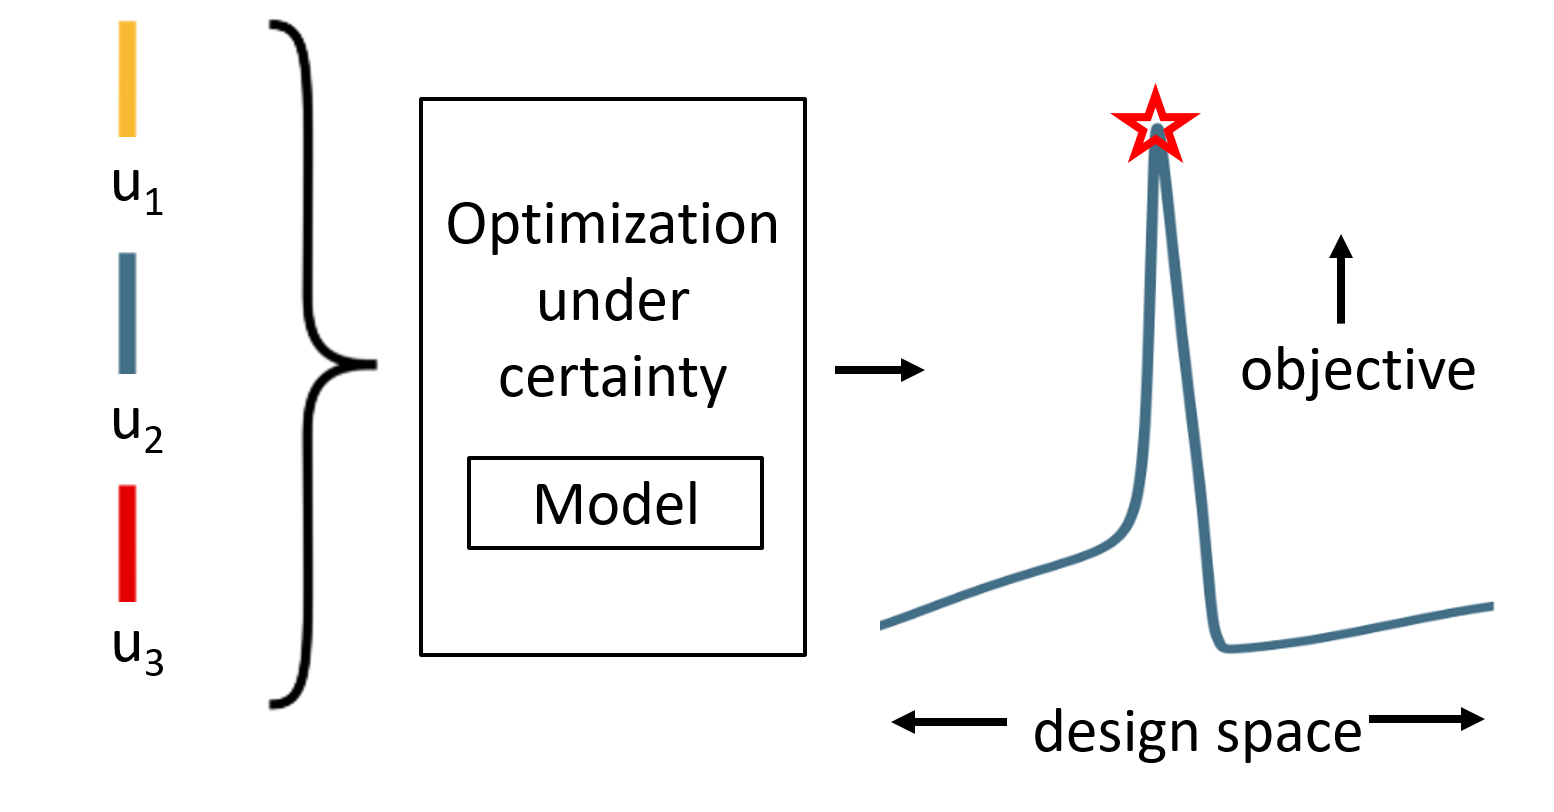
\includegraphics[width=.8\linewidth]{ouc.PNG}
    \end{subfigure}
    \begin{subfigure}{.49\textwidth}
    \centering
        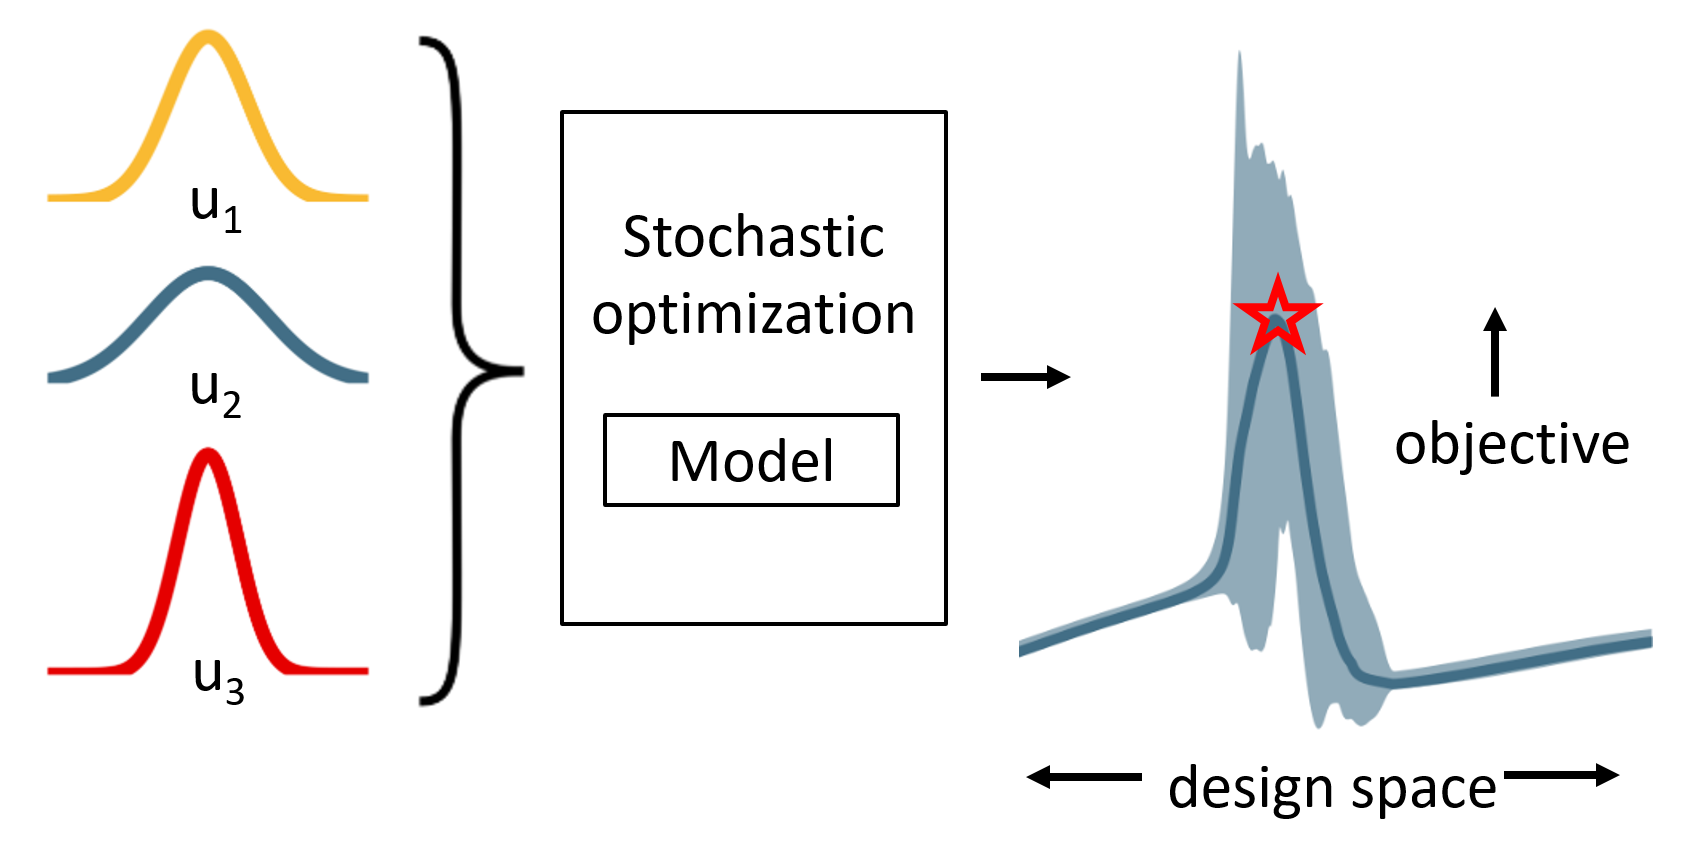
\includegraphics[width=.9\linewidth]{so.PNG}
    \end{subfigure}
    \begin{subfigure}{.49\textwidth}
    \centering
        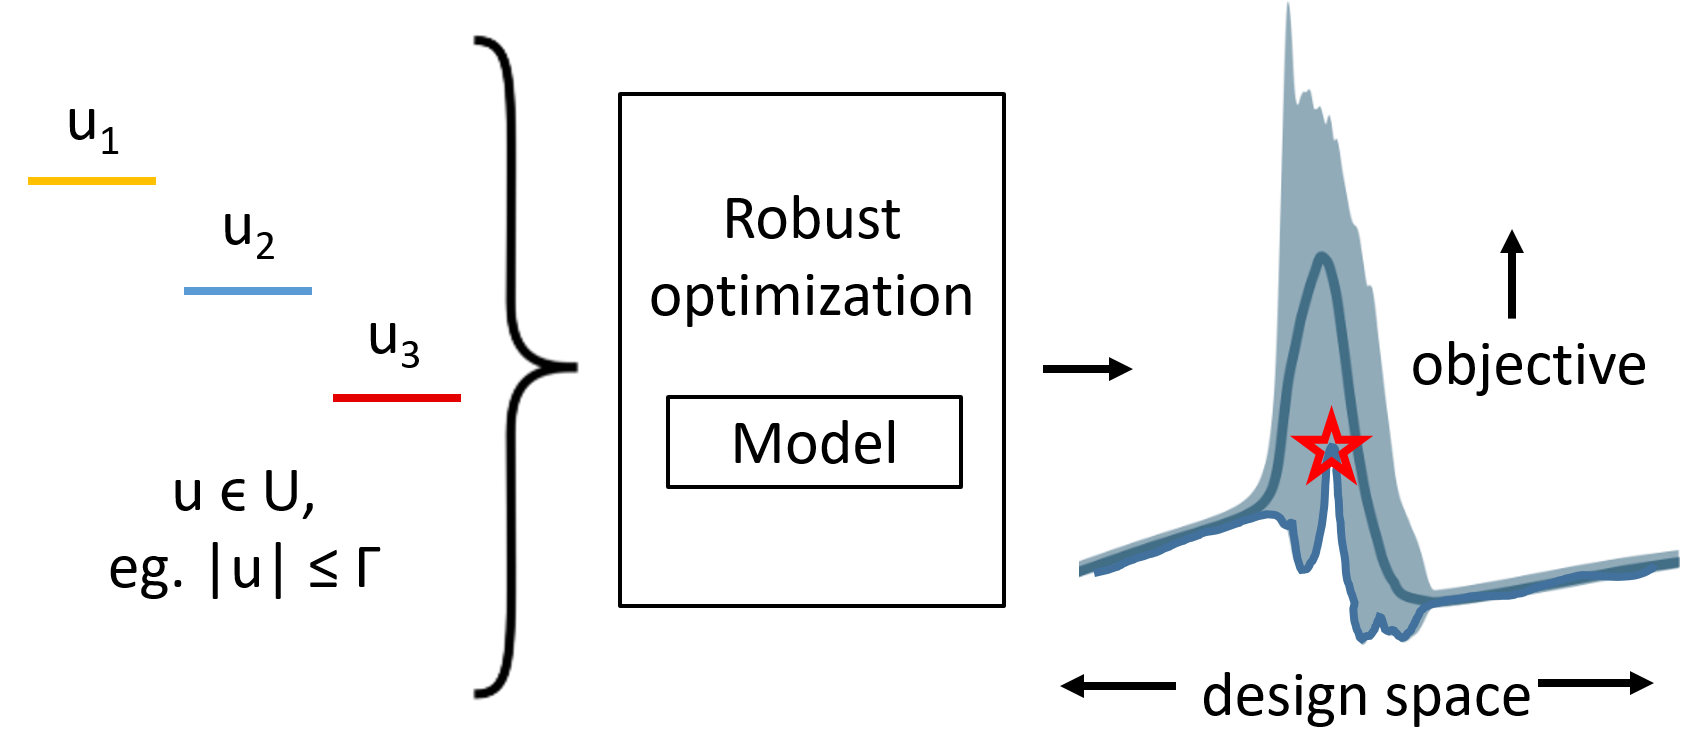
\includegraphics[width=.9\linewidth]{ro.PNG}
    \end{subfigure}
    \caption{\gls{so} and \gls{ro} are methods for optimization under uncertainty that use different definitions
             of uncertain inputs and produce different objective outcomes.}
    \label{fig:approaches}
\end{center}
\end{figure}

{\color{blue}\gls{so} pairs well with gradient-based approaches to solving nonlinear optimization problems
such as those defined in ~\cite{Gallard2013},~\cite{Liem2015} and ~\cite{Liem2017}.
These approaches implement an iterative process where
the objective function and constraints are evaluated over an initial design, and first- and/or
second-order information are used to converge the design towards a local optimum.
In this context, \gls{so} problems deal with uncertainty by including
probability distributions of the uncertain parameters in the iteration, and propagating
the distributions through the physics of a design problem to ensure constraint feasibility with certain probability.
The predominant goal of \gls{so} is to optimize some distributional
characteristics, eg. the mean as in Figure~\ref{fig:approaches},
of the probability density function of the objective~\cite{Diwekar2008}.}

{\color{blue}There have been recent developments in multi-mission aircraft design
using \gls{so}.
Liem et. al~\cite{Liem2015} propose the use of optimally
weighted objective functions over an aircraft's operational
design envelope for robust aircraft design.
In following work, Liem et al. generate probability distributions
of uncertain parameters from data
and minimize the expectation of an objective function over
parameter distributions~\cite{Liem2017}.
Although these stochastic methods demonstrate significant improvements over
legacy design methods in terms of design robustness,
they do not address many of the aforementioned challenges of legacy design methods
in capturing the robustness-optimality tradeoff.
The scope of the design problems is narrow and limited to aerostructural optimization,
and the number of uncertain parameters is low.
The formulations assume the presence of data, limiting the
effectiveness of the methods in conceptual design.
They have large computational costs that are somewhat mitigated through
surrogate modeling, but would be detrimental in the conceptual design phase.
Most importantly, they lack rigorous mathematical assessments of design feasibility
under uncertain parameters.}

In contrast to \gls{so},
\gls{ro} can only be applied to mathematical programs that have a robust counterpart,
such as linear, quadratic, semidefinite and geometric programs.
\gls{ro} takes a different approach than \gls{so} in both the form
of uncertain inputs and the objective functions. \gls{ro} produces designs that are
immune to constraint violations as long as parameter values come from within a defined
uncertainty set. The objective of \gls{ro} is to optimize the
the worst-case objective outcome of a design for a
given set over the uncertain parameters. As such,
\gls{ro} avoids the need to sample and propagate probability
distributions, and turns \gls{so} problems into
deterministic problems that are efficiently solved.}

\subsection{Comparison of robust and stochastic optimization methods for conceptual design}
\label{sec:robustvsstochastic}

Both \gls{ro} and \gls{so} have relative advantages in implementation. This paper will
argue specifically that the formulation of conceptual engineering design problems under uncertainty as
\gls{ro} problems has advantages over \gls{so} formulations (a more
mathematical programming centric comparison is made in~\cite{Bertsimas2011}).

\subsubsection{Generality and tractability}

In the context of engineering, we claim that an optimization method is general
when it can be used to solve a range of problems of interest. On the other hand,
tractability describes whether or not the problems are solved to a satisfactory
optimum within reasonable computational time. Optimization
under uncertainty is a difficult task that puts these two desirable subjective traits
at odds with each other.

\gls{so} has the advantage of generality.
\gls{so} methods are easily applicable to black box models or input-output systems.
They require little knowledge, if any, about the constraints in the system of interest.
\gls{ro} methods are less general, since they require
the design objective and constraints to be explicit and cast in a form that has a worst-case
counterpart. Thus models for \gls{ro} have to be transparent,
and \gls{ro} cannot be applied to black box models without significant prior data
manipulation and fitting at a minimum. A mitigating factor is that
many classes of conceptual engineering design problems can be cast or approximated in a form that
is compatible with robust optimization.

On the other hand, \gls{ro} is more tractable than \gls{so} due to the difference in method of uncertainty propagation.
As mentioned in Section~\ref{sec:sp},
\gls{so} methods involve the propagation of probability densities throughout a model
to determine their effects on constraint feasibility and the objective function.
This requires the integration of the product of probability distributions with potential outcomes,
and since the integration of continuous functions is difficult, this is often achieved through
a combination of high-dimensional quadrature and discretizations of the uncertainty into
possible scenarios. This propagation method
results in a combinatorial explosion of possible outcomes which need to be evaluated to determine constraint
satisfaction and the distribution of the objective. As a result, few problems can be addressed purely
through \gls{so}
(eg. recourse problems~\cite{Kall1982},\cite{Higle1991}; the energy planning problem~\cite{Pereira1991};
and certain aircraft design problems ~\cite{Liem2015},\cite{Liem2017}), and
even these are limited by combinatorics and costly system evaluations. Furthermore, they require
problem-specific approximations, so that generality is compromised.
Robust versions of tractable optimization problems are not
guaranteed to be tractable, but in practice the aforementioned classes of optimization problems
have tractable robust formulations~\cite{Bertsimas2011}. In \gls{ro},
there are no separate optimization and evaluation
loops by construction, and thus \gls{ro} problems can be solved to optimality
many orders of magnitude faster than \gls{so} problems of the same form~\cite{Bertsimas2011}.

Conceptual design optimization values both generality and tractability, the former
because engineers would like to
apply methods for optimization under uncertainty without significant mathematical groundwork,
and the latter because fast solution times are critical
to reduce program risk early on in the design process when more aspects
of the design are fluid. From this perspective, the relative intractability of
\gls{so}-based approaches makes them unreliable for conceptual design, since significant time is
needed both to develop problem-specific tractable formulations, and to find satisfactory optima.
Furthermore,
many engineering design problems such as aircraft design are approximable by optimization
forms that have tractable robust counterparts, making \gls{ro} better suited
to conceptual design.

\subsubsection{Use of data}

\gls{so} problems generally require complete knowledge of the probability distribution of
parameters.
\gls{ro} requires only `modest assumptions  about distributions, such as a known mean and
bounded support'~\cite{Chen2007}. Since \gls{ro} does not require as much information
about uncertain parameters as \gls{so} does, it can better address conceptual design problems where there
is a lack of experience, or sparse and noisy data~\cite{Bertsimas2011}. It is arguable that \gls{ro}
leaves a lot on the table by not taking advantage of distributional information,
however there is a growing body of research on distributionally robust optimization~\cite{Bertsimas2018}
which seeks to leverage existing data.

\subsubsection{Stochasticity and probabilistic guarantees}

Although \gls{ro} problems solve problems with uncertainty,
\gls{ro} formulations result in \emph{deterministic}\footnote{Determinism in this case
refers to the outcomes of free variables in the optimization model.
Different instances of a deterministic design problem with
the same parameters will result in the same solution.} solutions that are immune
to all possible realizations of parameters in an uncertainty set~\cite{Bertsimas2011}.
There is extensive literature on \gls{ro} methods
that offer differing levels of conservativeness~\cite{Bertsimas2004}
depending on the kind of uncertainty set considered, that are guaranteed
to be feasible over the set of interest.

\gls{so} formulations provide no probabilistic guarantees
since the optimum depends on realizations of random variables\cite{Shmoys2004}.
This is not satisfactory from an engineering perspective, since
optimization runs over the same parameters may result in different
solutions. Furthermore, designs
can be sensitive to issues in sampling schemes over potentially unknown
probability distributions. In the context of engineering design, the determinism
and probabilistic guarantees of \gls{ro} makes
it superior to \gls{so}.

It is important to highlight that,
although both \gls{ro} and \gls{so} seek to address the problem
of optimization under uncertainty, they solve fundamentally different problems. In an ideal world where
we have a problem that is tractable and globally optimal for both methods, the two different
approaches would result in different solutions.

\subsection{Geometric and signomial programming for engineering design}

Geometric programming\footnote{Programming refers to the mathematical formulation of an optimization problem.}
is a method of log-convex optimization that has been developed
to solve problems in engineering design~\cite{Duffin1967}. Although theory of the \gls{gp} has existed since
the 1960's, \gls{gp}s have recently experienced a resurgence due to the advent of polynomial-time
interior point methods~\cite{Nesterov1994} and improvements in computing. They have been
applied to a range of engineering design problems with success. For a non-exhaustive list of examples,
please refer to~\cite{Boyd2007}.

\gls{gp}s have been effective in aircraft conceptual design
(\cite{Hoburg2013},~\cite{Burton2018}).
However, the stringent mathematical form of a \gls{gp} means it can only be applied to log-convex problems.
The \gls{sp} is the difference-of-log-convex extension of the \gls{gp} which can be applied to
solve this larger set of problems, albeit with the loss of some mathematical guarantees compared to the \gls{gp}~\cite{Kirschen2018}.
Aircraft pose some of the most challenging design problems~\cite{York2018}, and signomial programming
has been used to great effect in modeling and designing complex aircraft at a conceptual level quickly
and reliably as in \cite{York2018}, \cite{Kirschen2018} and \cite{Kirschen2016}.
Other interesting applications for SPs such as in network flow problems are being investigated.

Robust formulations exist for solving geometric programs with parametric uncertainty~\cite{Saab2018}.
The creation of a robust signomial programming framework to capture uncertainty in engineering
design, and specifically aircraft design, will allow us to have more confidence in the results
of the conceptual design phase, reduce program risk, and increase overall system performance.

\subsection{Contributions}

This paper proposes a tractable \gls{rsp} which we solve as a sequential \gls{rgp},
allowing us to implement robustness in non-log-convex problems such as aircraft design.
We extend the \gls{rgp} framework developed by Saab~\cite{Saab2018} to \gls{sp}s.
We implement the \gls{rsp} formulation on a conceptual aircraft design problem with over a hundred
variables as defined in~\cite{Ozturk2018}.
The benefits of \gls{ro} are demonstrated both in ensuring design feasibility and performance
using \gls{mc} simulations of the uncertain parameters.
We further explore the benefits of \gls{ro} in multiobjective optimization, and propose
a goal programming \gls{rsp} formulation for risk minimization problems.


